\section{Tetrachlorethan}

\subsection{Aufgabenstellung}

\begin{enumerate}
    \item Energie in Abhängigkeit des Diederwinkels zeichnen und die Anzahl der Min- bzw. Maxima bestimmen.
    \item Auswertung der erhaltenen Werte.
    \item Statistische Fehlerrechnung
    \item Vergleich der Methoden 
\end{enumerate}

\subsection{Diagramme von Tetrachlorethan}

Für Tetrachlorethan wurden, zur Bestimmung der Energie in Abhängigkeit des Drehwinkels, je zwei semiempirische und zwei ab-initio Methoden gewählt.
Zur Skalierung wurden wieder alle, durch HyperChem, erhaltenen Werte mit dem minimalsten Wert subtrahiert. Der zu erwartende Verlauf ist in Abbildung 4 zu sehen.
\vspace{1cm}

\begin{figure}[H]
    \centering
    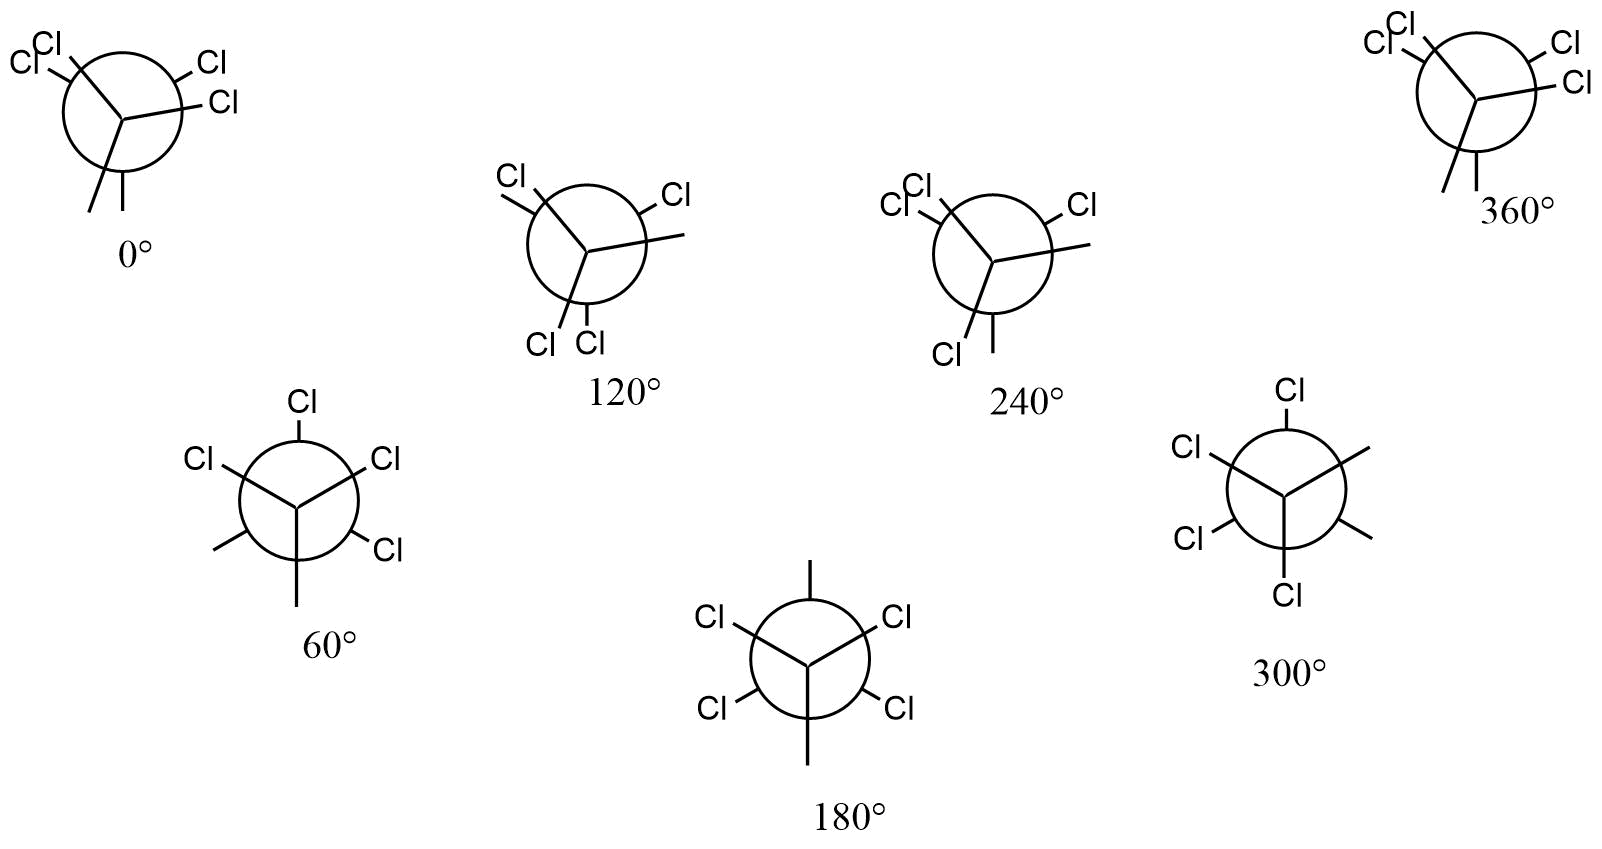
\includegraphics[scale=.3]{../src/img/newmanTetrachlorethan.png}
    \caption{Newman-Projektion von Tetrachlorethan}
\end{figure}

Der graphische Verlauf mit den Werten aus HyperChem sind in Abbildung 5 und 6 zu sehen.

\begin{figure}[H]
    \centering
    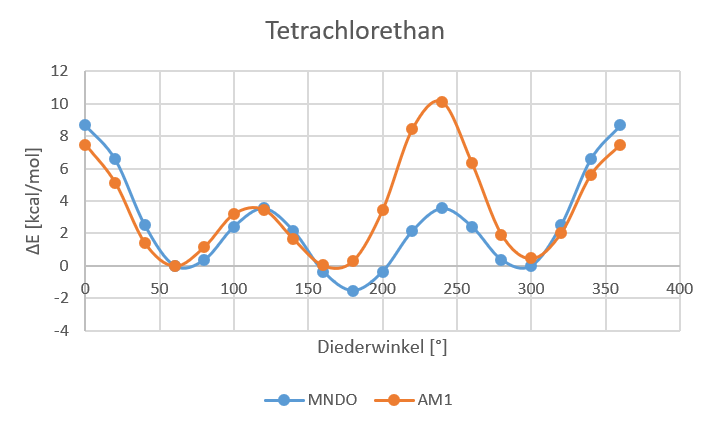
\includegraphics[scale=.7]{../src/img/tetrachlorethan1.png}
    \caption{Tetrachlorethan}
\end{figure}

Man kann sofort erkennen, dass die semiempirische AM1 Methode nicht für diese Aufgabenstellung geeignet ist, da der zu erwartende Verlauf (siehe Abbildung 4)
nicht eingehalten wird. Die anderen Methoden liefen ein für unsere Aufgabenstellung zu erwartendes Ergebnis, die globalen Maxima sind bei 0 bzw. 360$^\circ$ und das globale 
Minima befindet sich bei 180$^\circ$ (siehe Abbildung 4). \\



\begin{figure}[H]
    \centering
    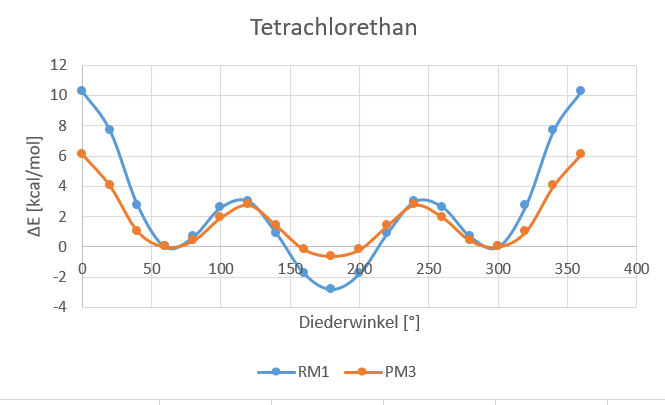
\includegraphics[scale=.7]{../src/img/tetrachlorethan2.png}
    \caption{Tetrachlorethan}
\end{figure}

\subsection{Auswertung der erhaltenen Werte}
Um die Methoden untereinander zu vergleich, wird wieder für die erhaltenen Werte, der Mittelwert, die Standartabweichung und die Präzision des Mittelwertes bestimmt.

% Table generated by Excel2LaTeX from sheet 'Eingabe'
\begin{table}[htbp]
  \centering
  \caption{Add caption}
    \begin{tabular}{lrrrrrrr}
    \toprule
    \textbf{Methode} & \multicolumn{1}{l}{\boldmath{}\textbf{$e^{el}_{min}$ [kcal/mol]}\unboldmath{}} & \multicolumn{1}{l}{\boldmath{}\textbf{$ZPE_{min}$}\unboldmath{}} & \multicolumn{1}{l}{\boldmath{}\textbf{$e^{el}_{max}$}\unboldmath{}} & \multicolumn{1}{l}{\boldmath{}\textbf{$ZPE_{max}$}\unboldmath{}} & \multicolumn{1}{l}{\boldmath{}\textbf{$\Delta e_{elec}$}\unboldmath{}} & \multicolumn{1}{l}{\boldmath{}\textbf{$\Delta ZPE$}\unboldmath{}} & \multicolumn{1}{l}{\boldmath{}\textbf{$\Delta e_{mol}$}\unboldmath{}} \\
    \midrule
    \textit{MNDO} & -1821,792 & 25,780 & -1819,042 & 25,710 & 2,749 & -0,070 & 2,679 \\
    \textit{AM1} & -3491,392 & 24,450 & -3490,575 & 24,310 & 0,818 & -0,140 & 0,678 \\
          &       &       &       &       &       &       &  \\
          &       &       &       &       &       &       &  \\
    \midrule
    \midrule
    \textit{Mittelwert} &       &       &       &       & 1,783 & -0,105 & 1,678 \\
    \textit{Stabw.} &       &       &       &       & 1,366 & 0,049 & 1,415 \\
    \textit{Präzision MW.} &       &       &       &       & 0,558 & 0,020 & 0,578 \\
    \bottomrule
    \end{tabular}%
  \label{tab:addlabel}%
\end{table}%
 

\subsection{Statistische Fehlerrechnung}

Für die statistische Fehlerrechnung wird, wie bei Ethan, die Formel der gauß'schen Fehlerfortpflanzung (Gl. 2) angewendet.

\begin{align*}
    \Delta e_{mol} &= \Delta ZPE + \Delta e^{el} \\
    \Delta e_{mol} &= 1.862 + 0.08 = \pm 1.942 \, [kcal/mol]
\end{align*}

\subsection{Vergleich der Methoden}

Wie schon in Teil 3.2 dargelegt, ist die Methode AM1 für dies Aufgabenstellung nicht anwendbar. Weiter fällt auf, dass die Energiewerte der ab-initio Methoden
bei den Maximas  größer und bei den Minimas kleiner sind, als die ihrer semiempirischen Pendants. Dies liegt wahrscheinlich an folgender Tatsache, da bei den ab-initio
Methoden zur Vereinfachung ideales Verhalten angenommen wird, werden kleinere Einflussfaktoren wie die intramolekularen Wechselwirkungen nicht mit einbezogen.
